%%
% このファイルは筑波大学情報学群情報科学類の卒業研究論文のサンプルです。
% このファイルを書き換えて、このサンプルと同様の書式の論文をLaTeXを使って
% 作成できます。
%
% OSやLaTeXの設定によっては漢字コードや改行コードを変更する必要があります。
%%
\documentclass[a4paper,11pt]{jreport}

\usepackage{xcolor}
%%【PDF, PostScript, JPEG, PNG等の画像の貼り込み】
%% dvipdfmx を使う場合
\usepackage[dvipdfmx]{graphicx}
%% dvipdfmx を使ってPDFの「しおり」を付ける場合
%%\usepackage[dvipdfmx,bookmarks=true,bookmarksnumbered=true,bookmarkstype=toc]{hyperref} \usepackage{pxjahyper}
\usepackage{ulem}
\usepackage{times} % use Times font instead of default one
\usepackage{algorithm}
\usepackage{algpseudocode}
\usepackage{amsmath}
\usepackage{url}
\usepackage{listings}

\lstset{
  language=Python,
  basicstyle=\ttfamily\small,
  commentstyle=\color{green},
  keywordstyle=\color{blue},
  stringstyle=\color{red},
  showstringspaces=false,
  numbers=left,
  numberstyle=\tiny\color{gray},
  numbersep=5pt,
  frame=tb
}

\setcounter{tocdepth}{3}
\setcounter{page}{-1}

\setlength{\oddsidemargin}{0.1in}
\setlength{\evensidemargin}{0.1in}
\setlength{\topmargin}{0in}
\setlength{\textwidth}{6in}
%\setlength{\textheight}{10.1in}
\setlength{\parskip}{0em}
\setlength{\topsep}{0em}

\newcommand{\figref}[1]{図\ref{#1}}
\newcommand{\tabref}[1]{表\ref{#1}}
\newcommand{\chapref}[1]{第\ref{#1}章}
\newcommand{\secref}[1]{\ref{#1}節}
\newcommand{\algorithmref}[1]{Algorithm \ref{#1}}
\newcommand{\equationref}[1]{式(\ref{#1})}
\newcommand{\appendixref}[1]{付録\ref{#1}}

%% タイトル生成用パッケージ(重要)
\usepackage{coins}

%% タイトル
\title{進化的計算による \ 輻輳制御アルゴリズムの探索手法の提案}
%% 著者
\author{岡部 純弥}
%% 指導教員
\advisor{岡 瑞起, 阿部 洋丈}

%% 年度と主専攻名
\fiscalyear{2023}
\majorfield{ソフトウェアサイエンス主専攻}

\begin{document}
\maketitle
\thispagestyle{empty}
\newpage

\thispagestyle{empty}
\vspace*{20pt plus 1fil}
\parindent=1zw
\noindent
%%
%% 論文の要旨
%%
\begin{center}
{\Large \bf 要  旨}
\vspace{2cm}
\end{center}

優れた輻輳制御アルゴリズムを発見することは難しい。主な理由として、コンピュータネットワークの構造が時々刻々と変化することが挙げられる。つまり、特定のネットワーク構造化で最適なアルゴリズムを探索しても、時間経過につれ、良いパフォーマンスを発揮できなくなってしまう。

そこで、大規模言語モデルと進化アルゴリズムを用いることで任意のネットワーク環境下で最適化を行う探索手法を提案する。
既存の探索手法では、探索空間の制約が厳しかったものの、大規模言語モデルを用いることで、この問題を解決できた。

実際にネットワークシミュレータを用いた実験を行い、ベンチマークを超える輻輳制御アルゴリズムを発見できた。

%%%%%
\par
\vspace{0pt plus 1fil}
\newpage

\pagenumbering{roman} % I, II, III, IV
\tableofcontents
\listoffigures
%\listoftables

\pagebreak \setcounter{page}{1}
\pagenumbering{arabic} % 1,2,3

\chapter{序論}

\section{研究背景}

TCP/IPネットワークでは、トランスポート層で輻輳制御が行われている。輻輳制御の難しさとして、限られた観測可能な値から、観測不可能な状態を推定しなければならないことが挙げられる。
つまり、限られた観測値から、輻輳が発生しているのかを判断したうえで、パケット送信量を制御しなければなければならない。

さらに、ネットワーク構造が変化し続けているため、支配的なアルゴリズムが存在することもなく、数年に一度はパラダイムシフトが起こっている。

現在の輻輳制御アルゴリズムの探索、発見は、ヒューリスティックに行われている側面があり、人的リソースを割き続けなければらない。つまり、ネットワーク構造の変化に柔軟に対応可能な探索手法の発見が求められている。

\newpage

\section{本論文の構成}

第2章の前半では、輻輳制御アルゴリズムの概要や、その発展について述べる。
第2章の後半では、近年の大規模言語モデルの発展や、その応用について概説する。特に、輻輳制御アルゴリズムの探索手法として、大規模言語モデルを用いることの可能性について述べる。
第3章では、これらの関連研究を踏まえたうえでの仮説、および提案手法について述べる。
第4章では、仮説を検証するために提案手法の実装、実験の詳細について述べる。
第5章では、実験結果を示し、その結果に対する考察を行う。
第6章では、本論文のまとめと今後の課題について述べる。

\newpage

\chapter{関連研究}
\section{輻輳制御アルゴリズム}

\subsection{輻輳制御アルゴリズムの概要}

パケット交換型の通信網であるTCP/IPネットワークでは、トランスポート層で輻輳制御が行われている。
そもそも輻輳とは、ネットワーク上のあるノード
\footnote{多くの場合、これは中継ルータのいずれかである。}
で、パケットが過剰に蓄積されパケットロスが発生、あるいはパケットの遅延が発生する状態のことを指す。
一般的に、ルータ上ではパケットを蓄積するためのバッファが存在しており、これは FIFO: First In First Out 型のキューであるため、このバッファが溢れるとパケットのロスが発生する。
TCP/IPにおいて、トランスポート層では通信の信頼性を確保するために、パケットロスを検知するとパケットが再送される。
このため輻輳が発生すると、パケットロスが発生し通信のスループットが低下する。
\footnote{よりひどい状態になると、輻輳崩壊と呼ばれる状態になり、大規模な通信障害を引き起こすこともある。}
このような状態を回避するため
\footnote{Chiuら\cite{CHIU19891}は、単純な加算的増加、乗算的減少のアルゴリズムが、ネットワークの状態に関係なく効率的に輻輳回避に貢献することを検証した。}
に、輻輳制御という仕組みが存在する。

輻輳制御\cite{congestion-avoidance}は、観測可能な値からネットワークの状態を推定し、一度に送信するパケットの量を制御する。
多くの場合、輻輳制御によって輻輳の発生を抑えることができる
\footnote{実際にJacobson\cite{congestion-avoidance}で提案された、世界初の輻輳制御アルゴリズムは、TCP Tahoeと名付けられた。}
。万が一輻輳が発生した場合には、輻輳制御アルゴリズムは輻輳が発生していることを検知してパケット送信量を制御し、輻輳の影響を抑える。
興味深いことに、Kellyら\cite{kelly1998rate}は、全体最適化やゲーム理論の観点から、各々のノードが自身のパケット送信量を制御することでネットワーク全体としてのスループットを最大化できることを示した。
それゆえ現在の輻輳制御アルゴリズムは、OSのカーネルに実装されており、自分自身のパケット送信量を制御のみを行うことが多い。

単純な輻輳制御アルゴリズムの動作を\algorithmref{algorithm:congestion_control_algorithm}に示す。
\begin{algorithm}
  \caption{Basic Congestion Control Algorithm}
  \label{algorithm:congestion_control_algorithm}
  \begin{algorithmic}[1]
  \State $cwnd \gets 1$
  \State $ssthresh \gets veryLargeNumber$
  \While{true}
      \If{ACK is received}
        \If{$cwnd < ssthresh$}
            \State $cwnd \gets cwnd + 1$
        \Else
            \State $cwnd \gets cwnd \times 2$
        \EndIf
      \EndIf
      \If{Congestion is detected}
          \State $ssthresh \gets cwnd / 2$
          \State $cwnd \gets 1$
      \EndIf
  \EndWhile
  \end{algorithmic}
\end{algorithm}
\algorithmref{algorithm:congestion_control_algorithm}では、以下の2つの変数と、ACKの受信の契機によってパケットの送信量を調整する。

\begin{description}
  \item[cwnd] cwndは、一度に送信可能なパケットの数を表す。輻輳制御アルゴリズムは、このcwndを制御することで、パケット送信量を制御する。
  \item[ssthresh] ssthreshは、cwndを指数関数的に増加させる際の閾値を表す。ssthreshを超えた場合には、cwndは加算によって増加させる。
\end{description}
\algorithmref{algorithm:congestion_control_algorithm}では、輻輳が発生していない場合にはcwndを指数的あるいは線形に増加させることでパケット送信量を増加させる。
一方で輻輳が発生した場合には、cwndを減少させることで、パケット送信量を減少させる。
これが、輻輳制御アルゴリズムの基本的な動作である。

\subsection{代表的な輻輳制御アルゴリズム}

ここでは、代表的な輻輳制御アルゴリズムについて概説する。
輻輳制御アルゴリズムは、大きくLoss-basedとDelay-basedに分類される。
これは輻輳制御アルゴリズムがどのように輻輳を検知するかによって分類されており、Loss-basedはパケットロスを検知することで輻輳を検知する。
一方で、Delay-basedは、RTT: Round Trip Time
\footnote{パケットが送信元から受信元に送信され、さらにそのACKが送信元に返ってくるまでの合計時間のことを指す。}
を用いることで輻輳を検知する。
それぞれの代表的な輻輳制御アルゴリズムについて、\figref{figure:congestion_control_classification}に示す。
\begin{figure}[htbp]
  \centering
  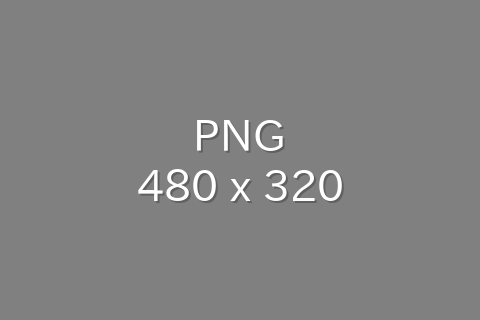
\includegraphics[width=0.6\linewidth]{fig/chap02/empty.png}
  \caption{[wip] 輻輳制御アルゴリズムの分類}
  \label{figure:congestion_control_classification}
\end{figure}
\figref{figure:congestion_control_classification} では、Loss-based 輻輳制御アルゴリズムをhoge色で、Delay-based 輻輳制御アルゴリズムをfuga色で示している。

\subsubsection*{Loss-based 輻輳制御アルゴリズム}

Loss-basedの代表的な輻輳制御アルゴリズムとしては、TCP Reno\cite{reno,tcp}が挙げられる。
これは、TCP Tahoe\cite{congestion-avoidance}を改良したもので、Fast RetransmitとFast Recoveryという機構を追加したものである。
これらはTCP Tahoeの課題であった、輻輳発生後のcwndの回復速度を改善するために追加された。
% TCP Renoの動作の概要を\figref{figure:reno-timeline}に示す。
% \begin{figure}[htbp]
%   \centering
%   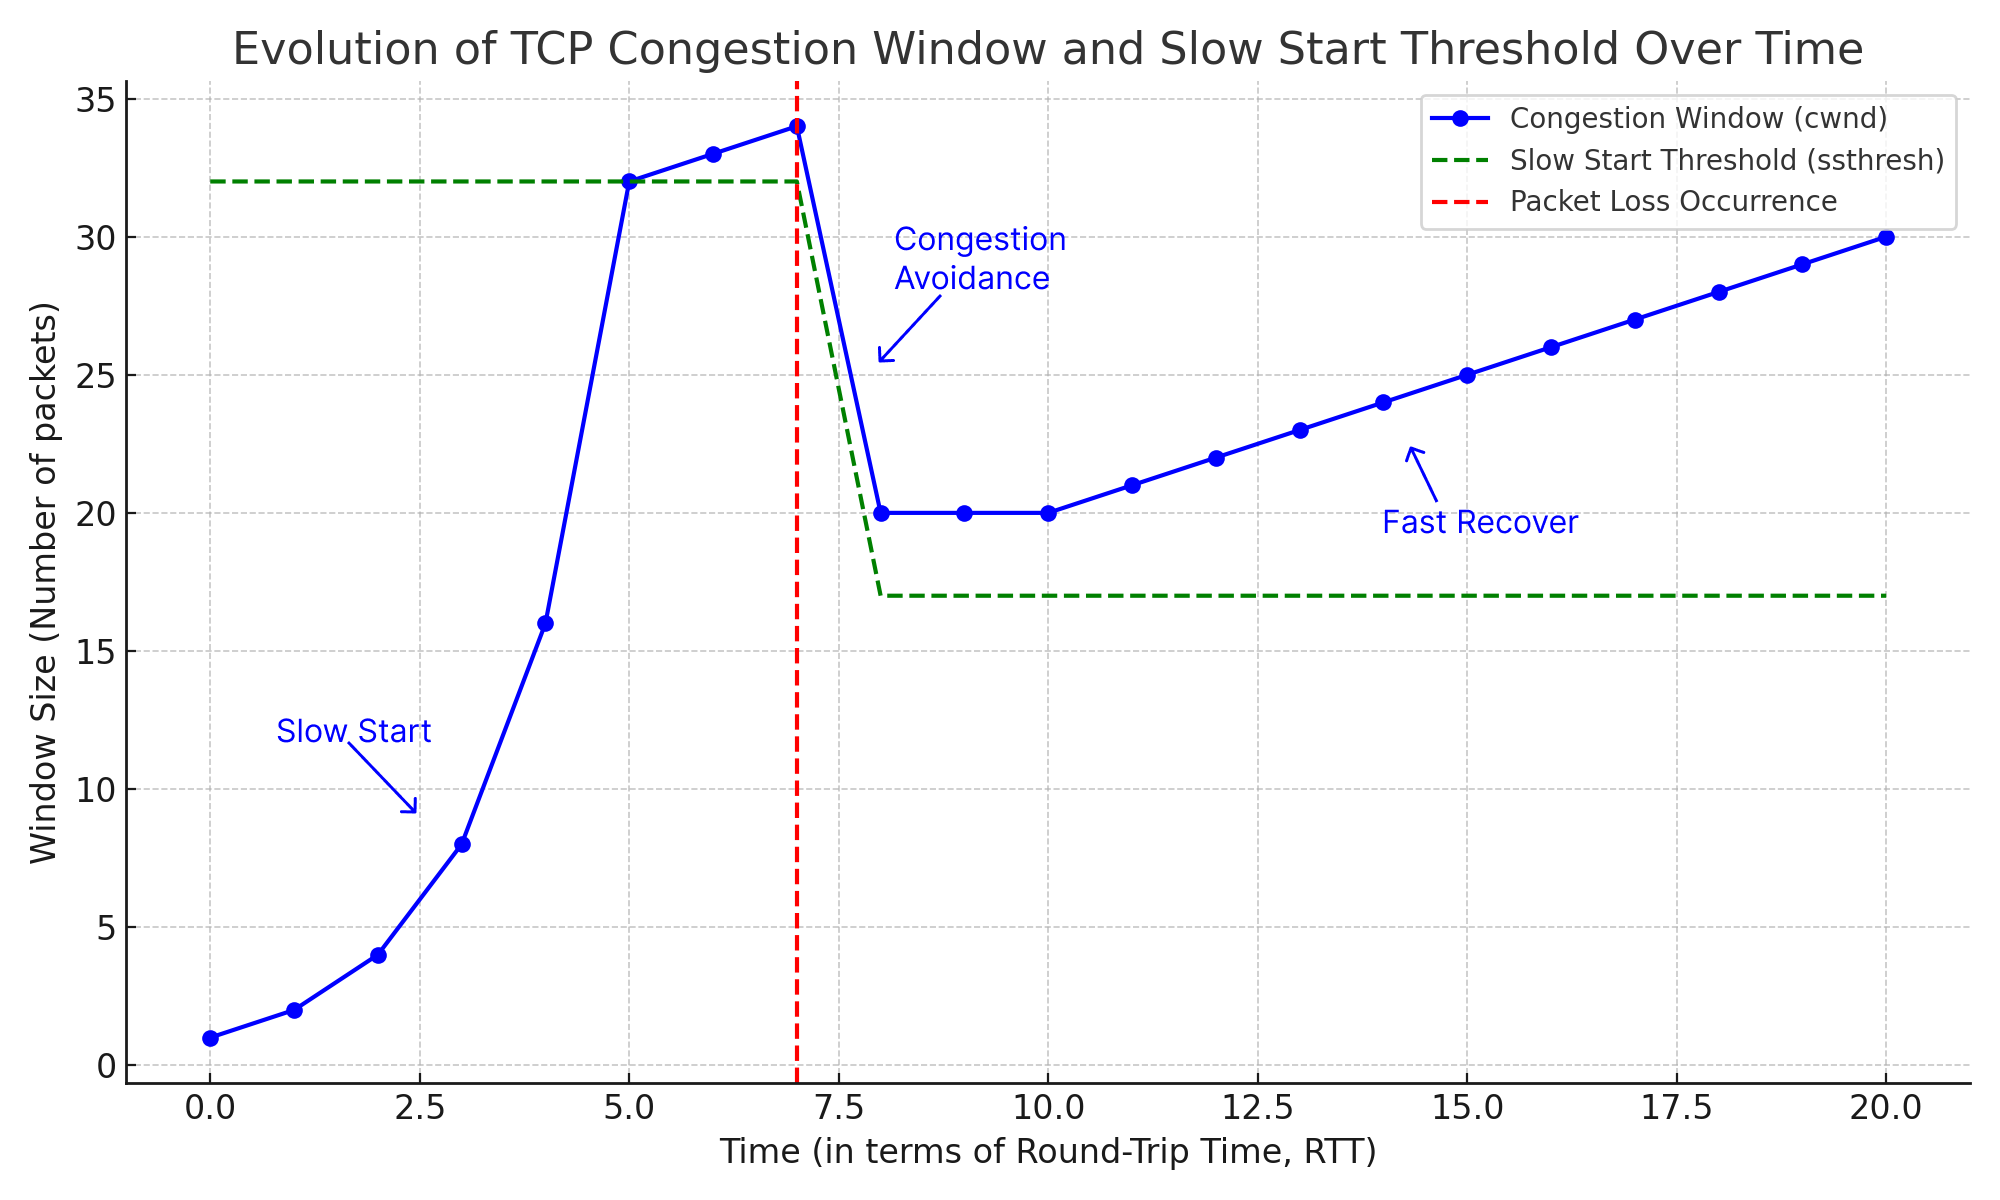
\includegraphics[width=0.6\linewidth]{fig/chap02/CongestionControlAlgorithm_Timeline.png}
%   \caption{TCP Renoの動作の概要}
%   \label{figure:reno-timeline}
% \end{figure}
% TODO: \figref{figure:reno-timeline}の説明

TCP Renoをさらに改良したTCP NewReno\cite{floyd2004newreno,henderson2012newreno}では、Fast Recoveryの実装やパケット損失時のcwndの回復方法が改良されている。
特に複数のパケットの損失時のcwndの回復方法が改良されている。
TCP RenoではFast Recover中に他のパケットが損失した場合、その損失は検出されず、ACKが受信されるまでcwndが回復しない。
一方で、TCP NewRenoではFast Recover中でも他のパケットに対する処理が行われるため、損失が検出されるとすぐにcwndが回復する。

その他の代表的なLoss-basedの輻輳制御アルゴリズムとしては、TCP Cubic\cite{cubic}が挙げられる。
Cubicは、ネットワークの帯域幅を効率的に利用するために、RenoやNewRenoを改良したものである。
特に、広帯域のネットワーク
\footnote{いわゆるロングファットパイプと呼ばれるネットワークである。}
において、Reno/NewRenoが帯域幅を効率的に利用できない問題があった。
Cubicでは、cwndの制御に三次関数を用いることで、これらの問題を解決している。
後述のBBR\cite{bbr}とともに、現代広く用いられている輻輳制御アルゴリズムである。

\subsubsection*{Delay-based 輻輳制御アルゴリズム}

一方で、Delay-basedの代表的な輻輳制御アルゴリズムとしては、TCP Vegas\cite{tcp-vegas}やBBR\cite{bbr}が挙げられる。
Delay-basedの輻輳制御アルゴリズムは、パケットロスを検知するのではなくRTTによってネットワーク上の輻輳の程度を推定し、パケット送信量を制御する。

TCP Vegasは、RTTの変化量を用いて輻輳を検出する。
RTTの変化による輻輳の検知は、一般的にはパケットロスによる検知よりも早いため、cwndの調整をより早く行うことができる
\footnote{実際には、Delay-basedな輻輳制御アルゴリズムの輻輳の検知がLoss-basedよりも早いことで、パフォーマンス上の問題が発生することがある。
例えばTCP Renoと、TCP Vegasが共存するネットワークにおいて、TCP VegasがRTTの変化によって素早くcwndを調整する一方で、TCP Renoはパケットロスが発生するまで、多くのパケットを送信し続ける。
それゆえ、帯域幅の多くをTCP Renoが占有することになり、TCP Vegasのパフォーマンスが低下することがある。
}
。それゆえ、帯域幅を効率的に利用することができる。
TCP Vegasのウインドウサイズの更新式を、\equationref{equation:tcp-vegas}に示す
\footnote{論文によっては、更新幅を1ではなく、$1/cwnd$としていることがある。
$1/cwnd$にすることで、$cwnd$が大きくなった際の更新幅を小さくし、輻輳の発生を抑制する効果がある。}。
ただし、$\alpha$と$\beta$は閾値を表す定数で、$\alpha \leq \beta$である。
\begin{equation}
  \label{equation:tcp-vegas}
  cwnd_{now} =
  \begin{cases}
    cwnd + 1 & \text{if } diff < \alpha \\
    cwnd - 1 & \text{if } diff > \beta \\
    cwnd & \text{otherwise}
  \end{cases}
\end{equation}
ここで、$diff$はRTTを元に推定される転送データの量であり、\equationref{equation:diff}に示すように計算される。
\equationref{equation:diff}の$RTT'$は、RTTの最小値を表す。
\begin{equation}
  \label{equation:diff}
  diff = \left( \frac{cwnd}{RTT'} - \frac{cwnd}{RTT}\right) RTT'
\end{equation}

BBR: Bottleneck Bandwidth and Round-trip propagation time は、Googleによって開発された輻輳制御アルゴリズムであり、従来の輻輳制御アルゴリズムとは異なるアプローチを採用している。
BBRでは、ボトルネックリンクの帯域幅
\footnote{経路上で最も低い値をとる帯域幅のことを指す。}
と往復時間遅延(RTproop: Round-trip propagation time)を推定し、これらの値を用いてパケット送信量を制御する。
BBRは、他のBBRを用いるノードとの通信において、公平性を保ちながら高いスループットと低遅延を実現できるためLinuxカーネル内でも実装されており、近年その採用が進んでいる。
一方で、他の輻輳制御アルゴリズムと共存した際に、BBRが帯域幅を占有する傾向にあることが指摘されている。

\subsubsection*{輻輳制御アルゴリズムの性能評価}
\label{section:congestion_control_algorithm_evaluation}

輻輳制御アルゴリズムの性能評価に関して、ネットワーク環境や評価指標など様々な観点から研究が行われている。
ネットワーク構造の変化や接続形態の変化、支配的な輻輳制御アルゴリズムの変化など多くの要因が輻輳制御アルゴリズムの性能に影響を与えるため、その評価は難しい。
輻輳制御アルゴリズムの性能評価について、Fallら\cite{fall1996simulation}は、SACK: Selective Acknowledgement ~\cite{rfc2018}を用いたシミュレーションに基づく輻輳制御アルゴリズムの性能を評価した。Moら\cite{752178}は、TCP Vegasの性能評価をネットワークの公平性の観点から行い、いくつかの改良点を提案した。

より詳細な輻輳制御アルゴリズムの概説や近年の研究の動向については、Lowら\cite{980245}やGhaffari\cite{GHAFFARI2015101}などを参照されたい。

\section{大規模言語モデルと進化アルゴリズム}

\subsection{大規模言語モデル}

近年、大規模言語モデルの発展が著しい。
自然言語処理の分野における機械翻訳のタスクは、もともとはRNN\cite{graves2014generating}やLSTM\cite{6795963}などの時系列モデルを用いて行われていた。
しかし、これらの手法では長期的な依存関係を捉えることが難しく、特に長い文章を高精度に翻訳できなかった。
2017年、Vaswaniら\cite{attention}の提案した、Transformerと呼ばれるモデルがこの問題を解決した。
Transformerは、Attentionと呼ばれる機構を用いて、長期的な依存関係を捉えることができる。
さらに、Transformerは、既存モデルと比べて並列化が容易であるため、学習にかかる時間を短縮できる。

さらに、Devlinら\cite{devlin2019bert}は、Transformerをベースとした、BERTと呼ばれる手法を提案した。
Brownら\cite{gpt3}は、GPT3と呼ばれるモデルを提案した。
これらのモデルは大規模なコーパスを用いて学習されており、様々なタスクで既存のモデルを凌駕する性能を発揮した。
現在では特にgpt3の系統のモデルを中心に、これらは大規模言語モデル(LLM: Large Language Model)と呼ばれており、自然言語処理の分野において、大きな影響を与えている。
また大規模言語モデルは、自然言語処理分野にとどまらず画像処理分野や音声処理分野などにも応用されている。

\subsection{進化アルゴリズム}

遺伝的アルゴリズム(GA: Genetic Algorithm)\cite{genetic-algorithm, vose1999simple}は、生物の進化を模倣したアルゴリズムであり、進化アルゴリズムの一種である。
特に最適化問題において、広く用いられている
\footnote{遺伝的アルゴリズムは古典的な手法であるため、多くの場合、より優れた探索手法が存在する。しかし、遺伝的アルゴリズムはその実装の容易さや、過去の研究の蓄積などから、最適化問題において広く用いられている。}
。
GAは、個体群の中から適応度の高い個体を選択し、交叉や突然変異といった進化演算子を用いて新たな個体を生成する。
一般的な進化演算子は以下のようなものがある。
\begin{description}
  \item[選択]
  個体群の中から、次世代に残す個体を選択する。多くの場合、適応度が高い個体ほど選択されやすい。
  \item[交叉] 2つの個体を選択し、それらの遺伝子を交換する。一様交叉や2点交叉などの方法がある。
  \item[突然変異] 遺伝子の一部をランダムに変更する。
\end{description}
遺伝的アルゴリズムは、これらの進化演算子を用いて個体群を進化させ、最適解を探索する。
より詳しい遺伝的アルゴリズムの総説や、近年の応用については、Katochら\cite{katoch2021review}を参照されたい。

\subsection{進化アルゴリズムへの大規模言語モデルの応用}

近年、大規模言語モデルを用いて、進化アルゴリズムの進化演算子を実現する研究が行われている。Meyersonら\cite{meyerson2023language}は、進化演算における交叉を大規模言語モデルを用いて実現できるのかを検証し、いくつかの分野の問題
\footnote{数式生成のタスクや、画像処理、ソースコードの生成など}
において、これがうまく機能することを示した。
Lehmanら\cite{lehman2022evolution}は、大規模言語モデルを用いた変異によって、進化アルゴリズムがうまく機能するかを検証し、これを示した。

つまり単純なタスクであれば、進化アルゴリズムにおける交叉や変異を、大規模言語モデルを用いて実現できることが示されている。
特に変異においては、大規模言語モデルを用いることで、従来の手法より探索空間が広がりやすく、より多様な解を探索できることが示されている。

\subsection{進化アルゴリズムの輻輳制御アルゴリズムへの応用}
\label{subsection:evolutionary-algorithm}

進化アルゴリズムや強化学習を用いて、輻輳制御アルゴリズムを探索する研究がいくつか行われている。
Endoら\cite{endo-2022-toward}は、遺伝的プログラミング\cite{holland1992adaptation, gp, gp-foundation}
\footnote{厳密には、GE (Grammatical Evolution) \cite{grammatical-evolution}と呼ばれる、遺伝的プログラミングの一種を用いている。GE では、プログラムの文法をBNF (Backus-Naur Form) で表現し、定義された文法に従ってプログラムを生成する。}
と品質多様性アルゴリズム\cite{quality-diversity}、共進化アルゴリズム\cite{poet, poet-gecco}を用いた輻輳制御アルゴリズムの探索を行った。

Endoらの研究では、実行可能な輻輳制御アルゴリズムを探索することに成功していたものの、遺伝的プログラミングを用いていたため、探索空間が限定されていたという問題があった。
Endoらの研究に限らず、遺伝的プログラミングや強化学習を用いた輻輳制御アルゴリズムの探索では、探索空間が限定されていることが多い。
これは文法をあらかじめ定義していることや、交叉や変異がAST: Abstract Syntax Treeに対する操作に限定されていることが原因である。
この問題に対する解決策を次章で検討する。

\newpage

\chapter{仮説}
\label{chapter:hypothesis}
関連研究をもとに、以下の仮説を立てた。
\begin{enumerate}
  \item 大規模言語モデルを用いた輻輳制御アルゴリズムの探索手法は、既存の探索手法と比べて、探索空間が広がるのではないか
  \item 進化アルゴリズム、特に遺伝的アルゴリズムを用いることで、既存の探索手法よりも多様かつ優れた輻輳制御アルゴリズムを発見できるのではないか
  \item 1, 2で提案した探索手法であれば、任意のネットワーク環境下
  \footnote{実験を行うネットワークシミュレータ上で環境を再現できる場合に限り}
  で最適な輻輳制御アルゴリズムを発見できるのではないか
\end{enumerate}
つまり、``大規模言語モデルを用いて交叉や変異を行う遺伝的アルゴリズムを用いて、輻輳制御アルゴリズムを探索する''という探索手法を提案する。
提案手法の概要を\figref{figure:proposed_flow}に示す。
\begin{figure}[htbp]
  \centering
  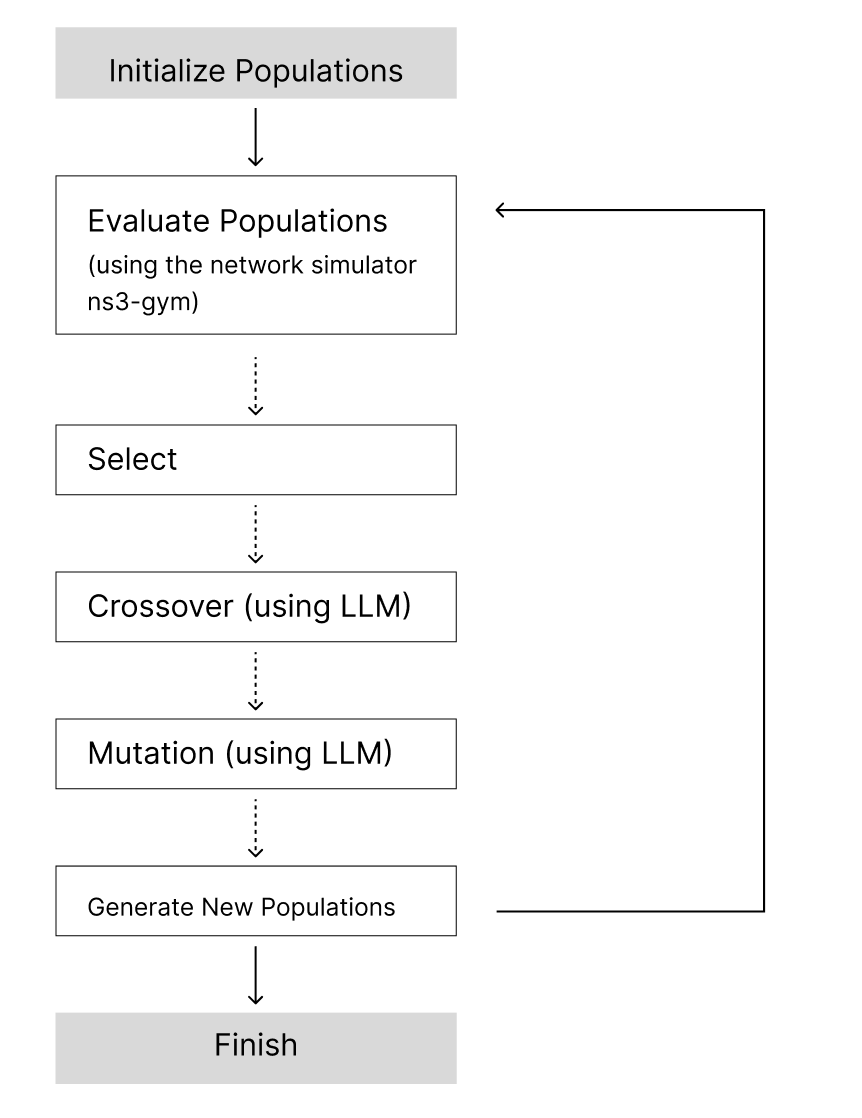
\includegraphics[width=0.4\linewidth]{fig/chap03/proposed_flow.png}
  \caption{提案手法の概要}
  \label{figure:proposed_flow}
\end{figure}
この提案手法は、既存の探索手法よりも、探索空間が広がり多様かつ優れた輻輳制御アルゴリズムを発見できるのではないか。

ソースコードで表現されるアルゴリズムを進化計算によって探索する場合、遺伝的プログラミング(GP: Genetic Programming)が用いられることが多い。
しかしGPでは、ソースコードを木構造によって表現しており、交叉や変異は木構造に対する操作となるため、探索空間が厳しく制限されてしまう。
変異によって木構造の一部が別の木構造に置き換えられることがあるが、それでも探索空間は制限されてしまう。

大規模言語モデルを用いた交叉や変異は、この探索空間上の制約が緩和されるのではないか。
さらに、特に変異において、有意な変化が起こる確率が高くなるのではないか。
この仮説を検証するために、大規模言語モデルを用いた遺伝的アルゴリズムを実装し、ネットワークシミュレータns3\cite{ns3-2012, ns3-2010}を拡張したns3-gym\cite{ns3gym}を用いて実験を行った。

\newpage

\chapter{実験}
\label{chapter:experiment}
この章では、実験の環境や実験方法、実装の詳細やその評価方法について述べる。

\section{実験環境}

\subsection{ネットワークシミュレータ}

本研究ではネットワークシミュレータとして、ns3-gym\cite{ns3gym}を用いた
\footnote{厳密に言えばns3-gymは、OpenAI Gymとns3のインタフェースを提供するフレームワークである。しかしここでは簡単のため、単にネットワークシミュレータと呼ぶ。}。
ns3-gymは、ns3\cite{ns3-2012, ns3-2010}を拡張したもので、OpenAI Gym\cite{gym}
\footnote{現在はOpenAI Gymの開発は終了しており、Gymnasium (\url{https://github.com/Farama-Foundation/Gymnasium}) への移行が進められている。}
のインターフェースを提供する
\footnote{つまり、ns3-gymでは輻輳制御アルゴリズムはPythonで表現され、これをns3のシミュレーションに組み込むことができる。
後述するOpenAIのgptモデルのAPI用ライブラリはPythonとnode.jsでのみ提供されているため、Pythonで実装されたns3-gymを用いた。
}。

そもそもns3とは、C++で実装されたネットワークシミュレータである。
ns3では、利用者が自由にネットワーク環境、プロトコルやアルゴリズムを設定し、ネットワークシミュレーションができる。
さらに、シミュレーション中にネットワークの状態を測定できる。
しかしns3では利用者が環境やプロトコルなどの大部分を設定、実装する必要があり、これらの設定や実装には多くの時間と知識が必要となる。
先述したとおり、ns3-gymはns3を拡張したものであるため、同様にネットワークシミュレーションができ、さらにシミュレーションのためのいくつかの一般的なネットワーク環境やシナリオが提供されている。
本実験では、この提供されている環境をベースに、輻輳制御アルゴリズムの探索実験を行った。実験に使用するネットワークトポロジーを\figref{figure:network-topology}に示す。
\begin{figure}[htbp]
  \centering
  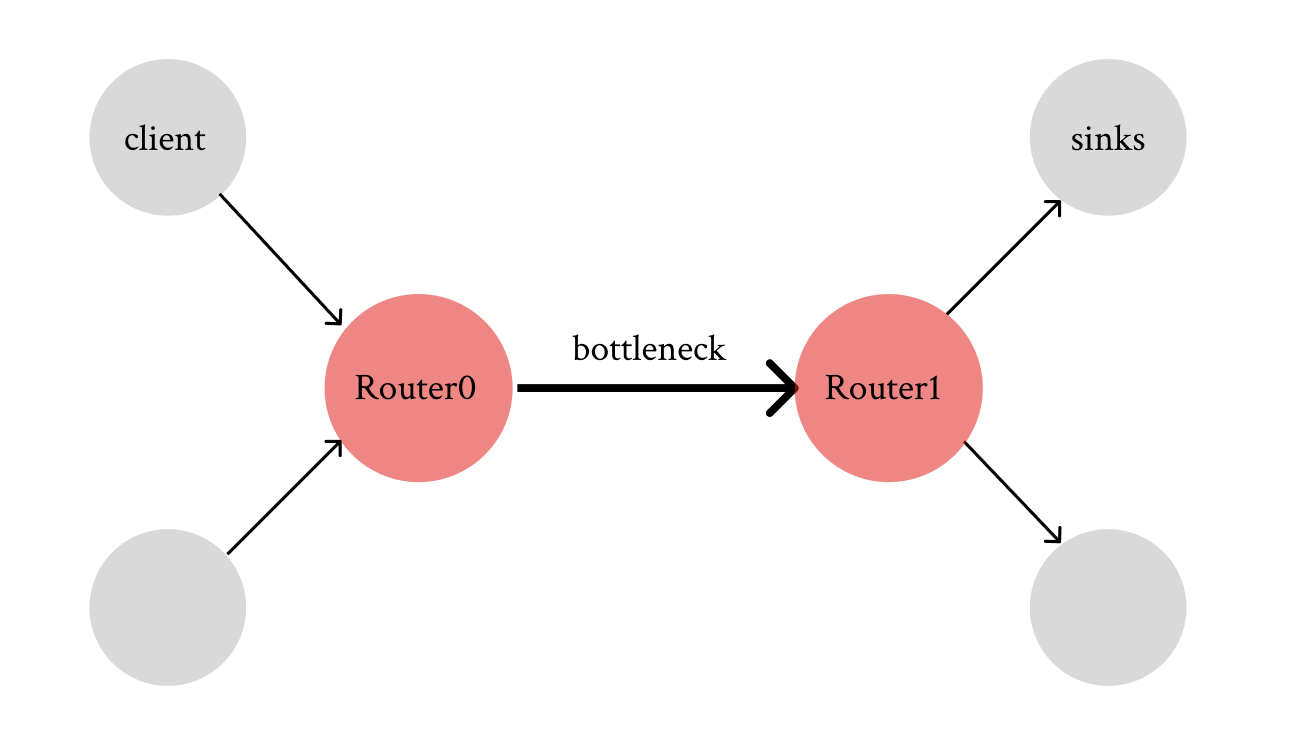
\includegraphics[width=0.6\linewidth]{fig/chap04/network-topology.png}
  \caption{ns3-gymで提供されるネットワークトポロジー}
  \label{figure:network-topology}
\end{figure}
\figref{figure:network-topology}は、いわゆるダンベル型のネットワークトポロジーと呼ばれるトポロジーである。
ダンベル型トポロジーでは、トラフィックはclientからsinks
\footnote{sinksは、ネットワーク上でのデータフローの終点を表す。}
へボトルネックリンクを介して流れる。
\secref{section:evaluation-method}で詳しく説明するが、本実験では\figref{figure:network-topology}のRouter1でスループットを計測することで、輻輳制御アルゴリズムの性能を評価する。

\subsection{大規模言語モデル}

本研究では、大規模言語モデルとしてOpenAIが提供するGPT-4を用いた。
GPT-4\cite{gpt4}は、2023年5月にリリースされたモデルで、多くのベンチマークでGPT-3\cite{gpt3}よりも高い性能を発揮している。
この実験を行っている2023年11月現在、OpenAIが提供するモデルの中ではもっとも性能が高いため、本研究ではGPT-4を用いる。
GPT-4はシンプルなJSON over HTTP(s) APIを提供している。
さらに、Pythonとnode.js用のAPI用ライブラリを公式に提供している。
したがって、本研究ではPythonを用いてPythonスクリプトからGPT-4のAPIを呼び出すことで、大規模言語モデルを利用する。

\subsection{実行環境}

本研究の実験は、以下のマシン上で行った。
また、Pythonのバージョンは3.11.6を用いた。

\begin{description}
  \item[CPU] Intel(R) Core(TM) i7-8700K CPU @ 3.70GHz
  \item[GPU] NVIDIA GeForce RTX 2080
  \item[メモリ] 64GB
  \item[OS] Ubuntu 22.04 LTS
\end{description}

\section{実験条件}
% ref. https://github.com/Okabe-Junya/ns3-gym/blob/master/scratch/rl-tcp/sim.cc

この節では特にネットワークシミュレータの設定について述べ、実験の条件を明らかにする。
本実験では、ネットワークシミュレータns3-gymのパラメータを\tabref{tab:network_simulator_parameters}に示すように設定した
\footnote{これらの設定は\url{https://github.com/Okabe-Junya/ns3-gym/blob/master/scratch/rl-tcp/sim.cc#L96-L111}で定義されている。ソースコードの該当箇所を直接書き換えるか、コマンドライン引数で上書きすることで設定を変更できる。}。
\begin{table}[ht]
  \centering
  \begin{tabular}{|l|l|}
  \hline
  \textbf{Parameter} & \textbf{Value} \\ \hline
  tcpEnvTimeStep & 0.01 \\ \hline
  nLeaf & 1 \\ \hline
  transport\_prot & TcpRl \\ \hline
  error\_p & 0.0 \\ \hline
  bottleneck\_bandwidth & 2Mbps \\ \hline
  bottleneck\_delay & 0.01ms \\ \hline
  access\_bandwidth & 10Mbps \\ \hline
  access\_delay & 20ms \\ \hline
  data\_mbytes & 0 \\ \hline
  mtu\_bytes & 400 \\ \hline
  duration & 10.0 \\ \hline
  flow\_monitor & false \\ \hline
  sack & true \\ \hline
  \end{tabular}
  \caption{ネットワークシミュレータの設定パラメータ}
  \label{tab:network_simulator_parameters}
\end{table}

\tabref{tab:network_simulator_parameters}の各項目について簡潔に説明する。
\begin{description}
  \item[tcpEnvTimeStep] ネットワークシミュレータにおける、TCP関連のイベントを発生させる間隔を表す。この値の間隔でウインドウサイズの更新やパケットの送信、再送信などが行われる。
  \item[nLeaf] ネットワークシミュレータにおける、TCPのリーフノード数を表す。厳密には、Routerの左右それぞれにnLeaf個のノードが接続される。今回はnLeaf=1であるため、\figref{figure:network-topology}のように、Routerの左右それぞれに1つのノードが接続される。
  \item[transport\_prot] トランスポート層で使用するプロトコルを表す\footnote{本実験で設定したTcpRlは、ns3-gymで提供されているトランスポート層のプロトコルの一つである。TCPを拡張し、強化学習が行えるように設計されているが、本実験の中ではTCPとは同様の挙動を示す。}。
  \item[error\_p] ネットワークでデータ転送中にエラーが発生する確率を表す。
  \item[bottleneck\_bandwidth] ボトルネックリンクの帯域幅を表す。
  \item[bottleneck\_delay] ボトルネックリンクの遅延を表す。
  \item[access\_bandwidth] アクセスリンクの帯域幅を表す。ただしアクセスリンクとは、エンドユーザがネットワークへ接続する際に使用するリンクのことである。
  \item[access\_delay] アクセスリンクの遅延を表す。
  \item[mtu\_bytes] 最大転送速度(MTU: Maximum Transmission Unit)のバイト数を表す。これは一度に送信できるパケットの最大サイズを表す。
  \item[duration] シミュレーションの実行時間を表す。
  \item[flow\_monitor] フローモニタを有効にするかどうかを表す。フローモニタとは、ネットワークシミュレータにおいて、データフローを追跡するためのモジュールである。
  \item[sack] SACK: Selective Acknowledgement を有効にするかどうかを表す。一般的にはこれを有効にすることで、TCPの性能が向上する。
\end{description}


\section{実験方法}
\label{section:experiment-method}
この節では実験の方法について述べる。
方針は、\chapref{chapter:hypothesis}の\figref{figure:proposed_flow}で示したように、輻輳制御アルゴリズムを個体として、遺伝的アルゴリズムによって探索することである。
このとき、遺伝的アルゴリズムの交叉や変異は、大規模言語モデルを用いて実現する。
評価関数については、\secref{section:evaluation-method}であらためて述べる。
実験で実装する遺伝的アルゴリズムの擬似コードを\algorithmref{algorithm:genetic-algorithm}に示す。
\begin{algorithm}[htbp]
  \caption{Pseudocode of Genetic Algorithm}
  \label{algorithm:genetic-algorithm}
  \begin{algorithmic}[1]
    \Require
      \Statex $N$: Population size
      \Statex $G$: Number of generations
      \Statex $P$: Crossover probability
      \Statex $M$: Mutation probability
      % \Statex $L$: Length of chromosome
      \Statex $f$: Evaluation function
    \Ensure
      \Statex $best$: Best individual in population

    \State $population \gets$ Initialize population
    \For{$g \gets 1$ to $G$}
      \State $population \gets$ Evaluate population using $f$
      \State $best \gets$ Best individual in $population$
      \State $nextPopulation \gets$ $\phi$
      \State $p1$ $\gets$ select $population$
      \State $p2$ $\gets$ select $population$
      \For {$i \gets 1$ to $N$}
        If {random() $<$ 0.5}
          c $\gets$ $p1[i]$
        Else
          c $\gets$ $p2[i]$
        EndIf
        \If {random() $<$ $P$}
          c $\gets$ crossover($p1[i]$, $p2[i]$)
        \EndIf
        \If {random() $<$ $M$}
          c $\gets$ mutate(c)
        \EndIf
        \State $nextPopulation \gets nextPopulation \cup \{c\}$
      \EndFor
      \State $population \gets nextPopulation$
    \EndFor
  \end{algorithmic}
\end{algorithm}
本実験では、\algorithmref{algorithm:genetic-algorithm}に示した疑似コードを実際にPythonで実装し、実験を行った。

\section{評価方法}
\label{section:evaluation-method}

遺伝的アルゴリズムの評価関数として、\figref{figure:network-topology}のRouter1で計測されるスループットを用いた。
\secref{section:evaluation-method}で述べたとおり、遺伝的アルゴリズムの各個体は輻輳制御アルゴリズムを表すPythonスクリプトであるため、これをネットワークシミュレータに組み込んで実行することで、その性能を評価できる。
0.01秒ごとにRouter1で計測されたスループットを取得し、その平均値を評価関数とした。
時刻$t$におけるスループットを$T(t)$とすると、評価関数$f$は\equationref{equation:evaluation-function}のように表される。
\begin{equation}
  \label{equation:evaluation-function}
  f = \frac{1}{N} \sum_{t=0}^{N} T(t)
\end{equation}
ただし\equationref{equation:evaluation-function}で、$N$はスループットの計測回数を表す。

\newpage

\chapter{結果}

\label{chapter:result}
\chapref{chapter:experiment}で説明した実験を行った。
この章では、その実験結果を示す。
\figref{figure:generation_throughput}に、遺伝的アルゴリズムの世代ごとの評価値
\footnote{評価値は、\secref{section:evaluation-method}で述べた評価関数$f$の値である。}
の平均、最大値の推移を示す。
\figref{figure:generation_throughput}で、横軸は世代数、縦軸はスループットを表す。
ここでGAの交叉や変異によって実行不可能なアルゴリズムが生成された場合、その評価値は0となる。
その影響を減らすために、評価値の上位50\%の個体のみを用いた平均も合わせて示す。
\begin{figure}[thbp]
  \setlength\fboxsep{0pt}
  \centering
  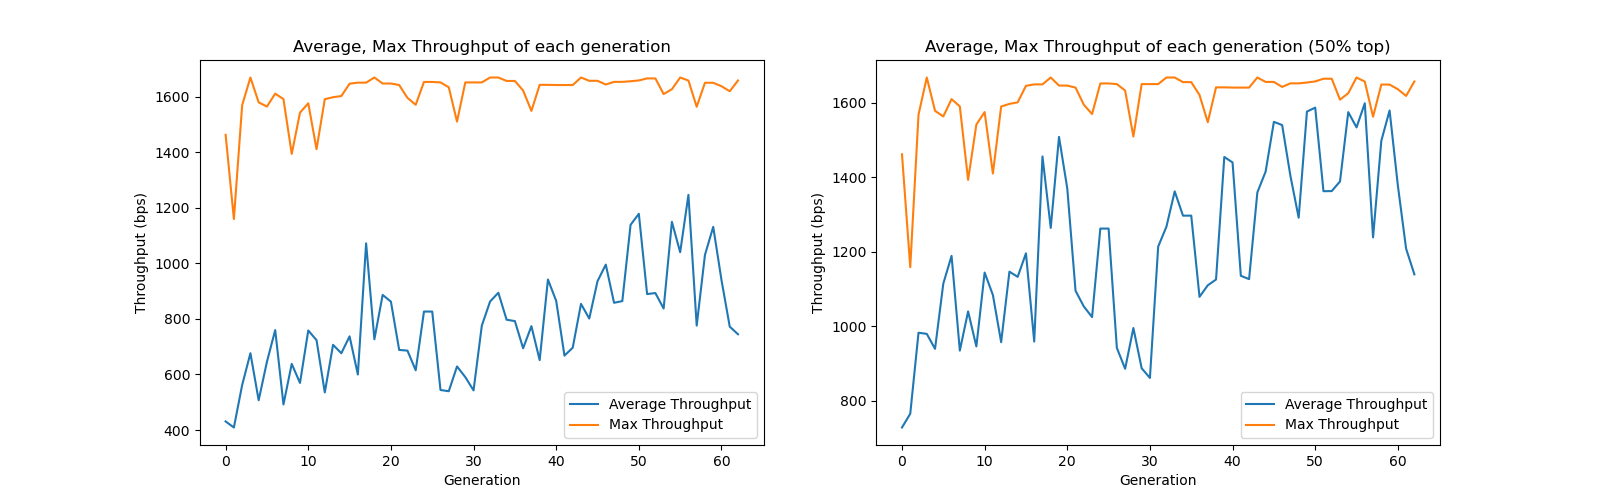
\includegraphics[width=0.9\linewidth]{fig/chap05/generation_throughput.png}
  \caption{世代ごとのスループットの平均、最大値の推移}
  \label{figure:generation_throughput}
\end{figure}
\figref{figure:generation_throughput}から、世代が進むにつれて、評価値の平均が緩やかな増加を示していることが読み取れる。
その一方、個体の評価値の最大値については、世代を追っても増加傾向は見られない。

実行不可能な個体を全て除いた場合の評価値の平均の推移を\figref{figure:generation_result_exclude_zero}に示す。
\begin{figure}[thbp]
  \setlength\fboxsep{0pt}
  \centering
  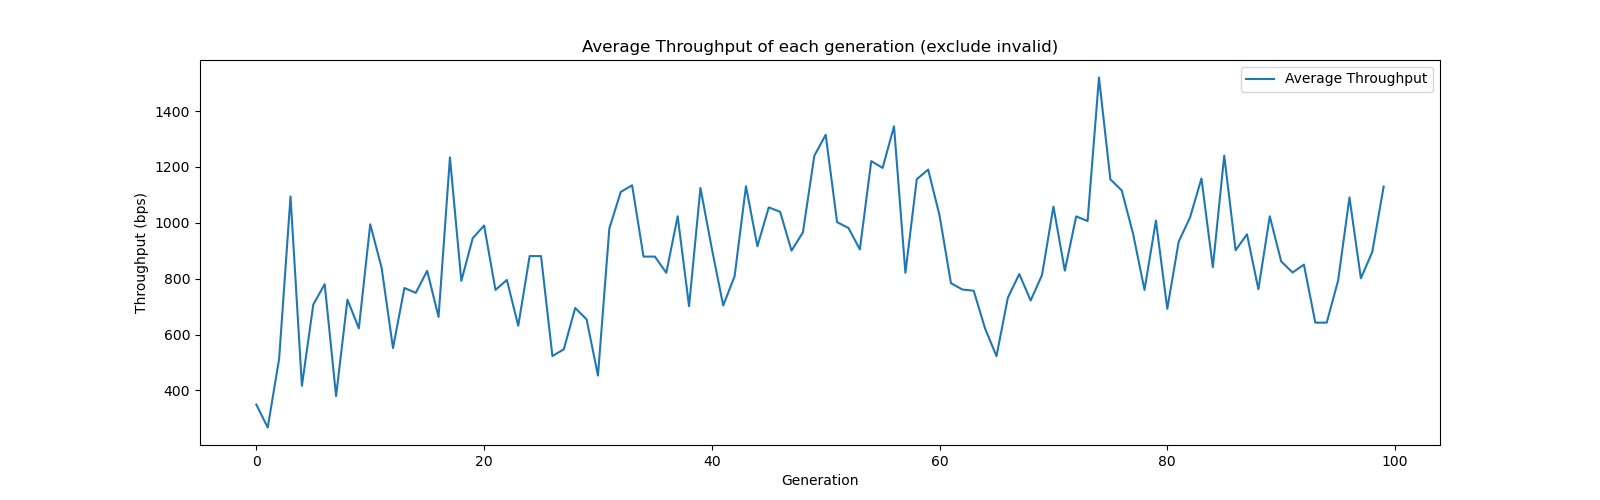
\includegraphics[width=0.9\linewidth]{fig/chap05/generation_throughput_exclude_zero.png}
  \caption{実行不可能な個体を除いた世代ごとのスループットの平均の推移}
  \label{figure:generation_result_exclude_zero}
\end{figure}
\figref{figure:generation_result_exclude_zero}を見ても、有意な増加傾向はあまり見られなかった。
これは、遺伝的操作である交叉や変異が、有効な個体を示していない可能性がある。
また、\figref{figure:invalid_results}に示すように、実行不可能な個体が少なからず生成されていた。
特に実行不可能な個体が多くされていた世代では、評価値の平均を取るための個体数が少なくなっており、平均値の推移にノイズが生じている可能性がある。

特定の世代における評価値の分布をより詳しく観察するために、1, 10, 50, 100世代の評価値の箱ひげ図を\figref{figure:boxplot_throughput}に示す。
\begin{figure}[thbp]
  \setlength\fboxsep{0pt}
  \centering
  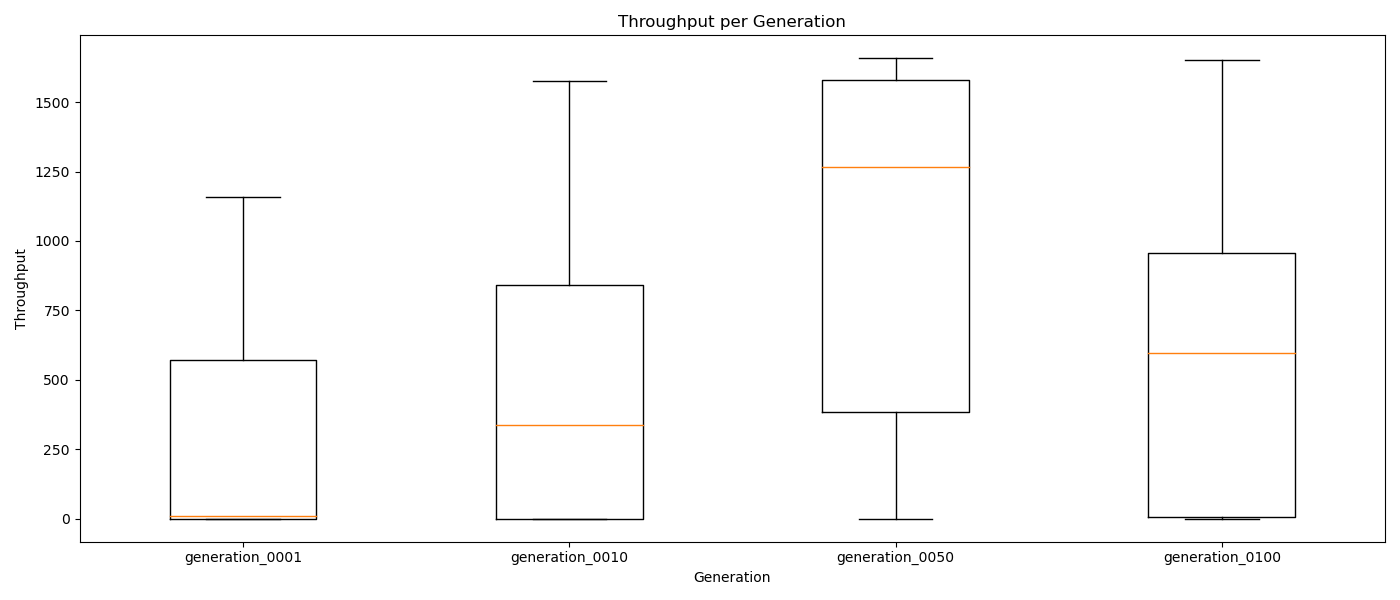
\includegraphics[width=0.9\linewidth]{fig/chap05/boxplot_throughput.png}
  \caption{1, 10, 50, 100世代のスループットの箱ひげ図}
  \label{figure:boxplot_throughput}
\end{figure}
\figref{figure:boxplot_throughput}を観察すると、100世代目を除くと、第一四分位点、中央値、第三四分位点は増加傾向にあることが読み取れる。
一方で、100世代目に注目すると、これらの値は減少しており、この間で探索がうまく行われなかった可能性がある。

評価値以外の個体の評価指標として、cwnd, ssthreshの平均の推移を観察する。
\figref{figure:generation_result}に、世代ごとのssthresh, cwndの平均の推移を示す。
\begin{figure}[thbp]
  \setlength\fboxsep{0pt}
  \centering
  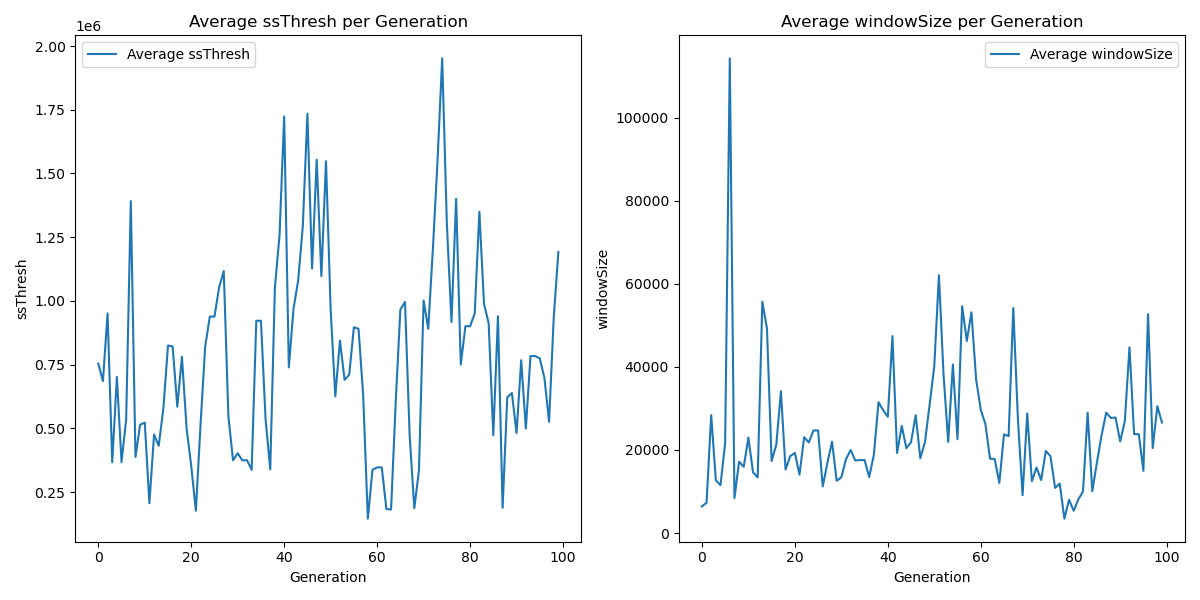
\includegraphics[width=1.0\linewidth]{fig/chap05/generation_result.png}
  \caption{世代ごとのssthresh, cwndの平均の推移}
  \label{figure:generation_result}
\end{figure}
\figref{figure:generation_result}を観察すると、世代を追っても、ssthresh, cwndの平均の推移に有意な変化は見られなかった。
もっとも、これらの値は、評価値とは異なる指標であるため、探索を進めても変化が見られないことは、必ずしも探索がうまく行われていないことを意味しないことに注意されたい。

評価値と同様、特定の世代におけるssthresh, cwndの分布をより詳しく観察するために、1, 10, 50, 100世代のssthresh, cwndの箱ひげ図を\figref{figure:boxplot}に示す。
\begin{figure}[thbp]
  \setlength\fboxsep{0pt}
  \centering
  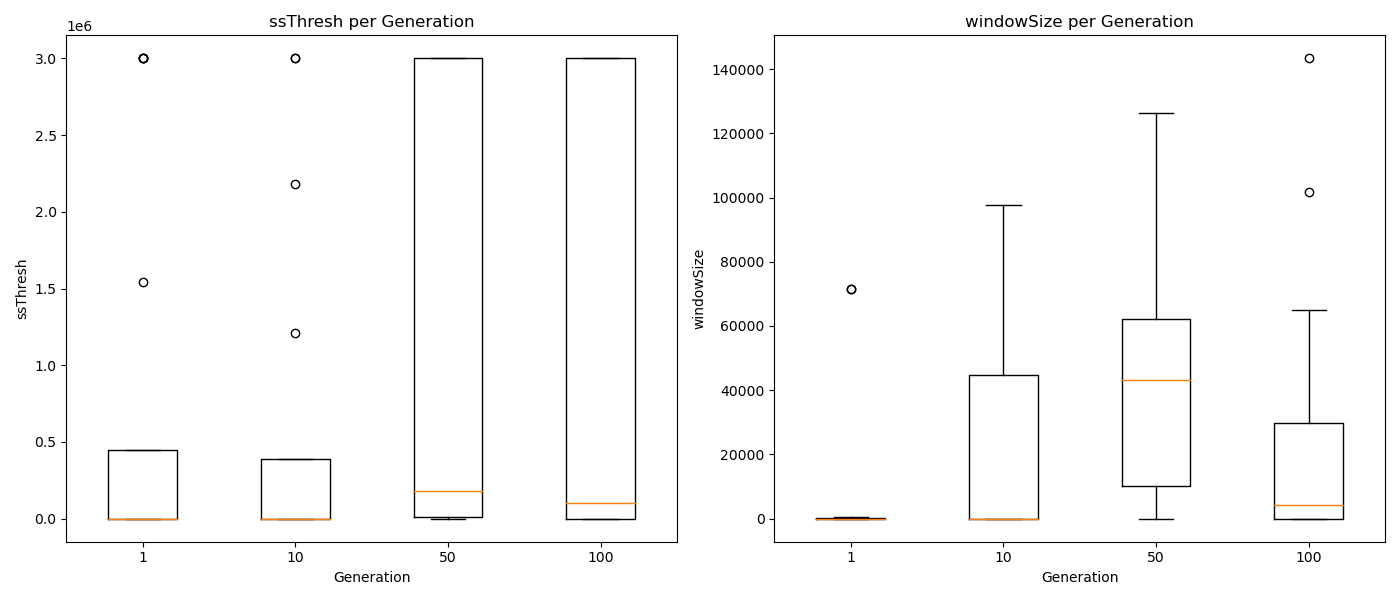
\includegraphics[width=1.0\linewidth]{fig/chap05/boxplot.png}
  \caption{1, 10, 50, 100世代のssthresh, cwndの箱ひげ図}
  \label{figure:boxplot}
\end{figure}
やはり箱ひげ図を観察しても、有意な変化は見られないことが読み取れる。

\newpage

個体の評価値やパラメータと異なる観点から、特に大規模言語モデルによる交叉や変異が機能していたかを確認するために、世代ごとに実行不可能な個体がいくつ生成されたかを可視化する。
ここで個体が実行不可能であるとは、以下のいずれかを満たすことを指す。
\begin{enumerate}
  \item 個体をネットワークシミュレータに組み込んで実行した際に、エラーが発生し、実行の終了コードが0以外となる
  \item 個体をネットワークシミュレータに組み込んで実行した際に、所定の時間内にシミュレーションが終了しない\footnote{本実験では、シミュレーションの実行時間を120秒として、この時間を超えてシミュレーションが終了しない場合は、実行不可能な個体とした。制限時間内に終了しない個体の多くは、極めて多くのパケットを送信し続ける個体であった。実際のネットワーク環境では、このような挙動を示す個体は実用的ではないこと、単に実験時間が必要以上にかかることから、今回は一定の制限時間を設けた。}
\end{enumerate}
\figref{figure:invalid_results}に、世代ごとの実行不可能な個体数の推移を示す。
\begin{figure}[htbp]
  \setlength\fboxsep{0pt}
  \centering
  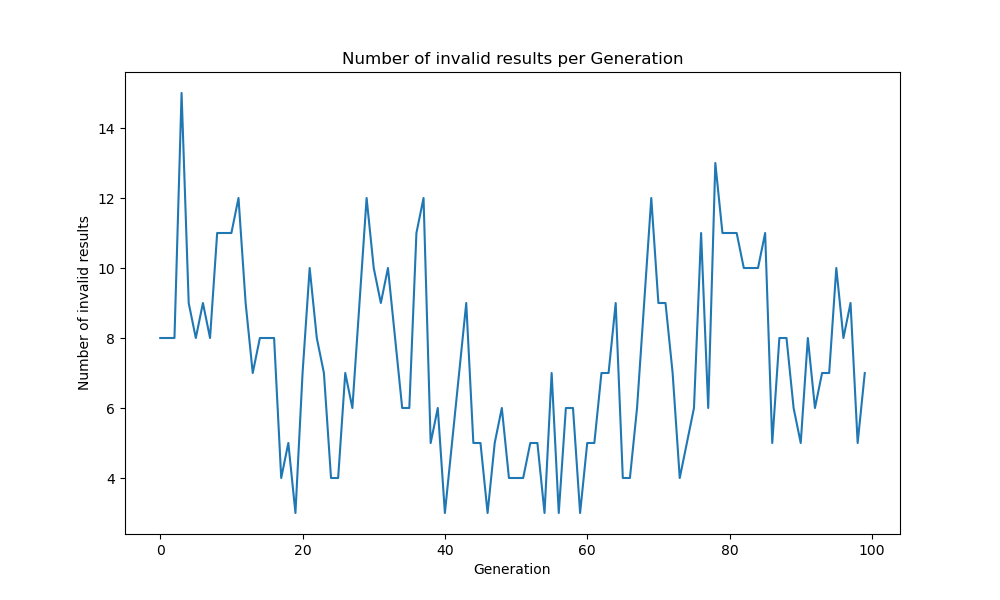
\includegraphics[width=1.0\linewidth]{fig/chap05/invalid_results.png}
  \caption{実行不可能な個体数の推移}
  \label{figure:invalid_results}
\end{figure}
\figref{figure:invalid_results}を観察すると、世代数と実行不可能な個体数には相関は見られないことが読み取れる。
また、\figref{figure:invalid_results}から、平均して約4割ほどの個体は実行不可能であり、交叉や変異によって少なからず実行不可能な個体が生成されていたことが確認できる
\footnote{実際、実行不可能な個体のうちの多くはタイムアウトによるものであった。特に、冪乗の計算や、乗算を繰り返すような個体は、多くのパケットを送信することになる。ns3-gymでは、実際に擬似的にパケットを送信するため、このような個体の実行には多くの時間がかかる。それゆえ、実行不可能な個体の多くは、タイムアウトによるものであった。}。

章の最後に、特定の個体について詳しく観察する。
全ての世代の中でもっとも高い評価値は、1668.45であった。
ベンチマークとして用いたNewRenoの評価値は1523.26であった。
したがって、本実験の環境下においては、もっとも高い評価値を示した個体はNewRenoよりも性能が高いと言える。
もちろん、実験環境やネットワークトポロジーによって、この結果は異なる可能性がある。
しかし本実験の環境は一般的なネットワーク環境を模したものであるため、この結果は一定の意味を持つと考えられる。
なお、もっとも高い評価値を示した個体のソースコードを\appendixref{appendix:experiment-result}のListings \ref{lst:best_individual}に示す。適宜参照されたい。

Listings \ref{lst:best_individual}の個体のシミュレーション中のssthresh, cwndの推移を\figref{figure:best_individual_result}に示す。
\begin{figure}[htbp]
  \centering
  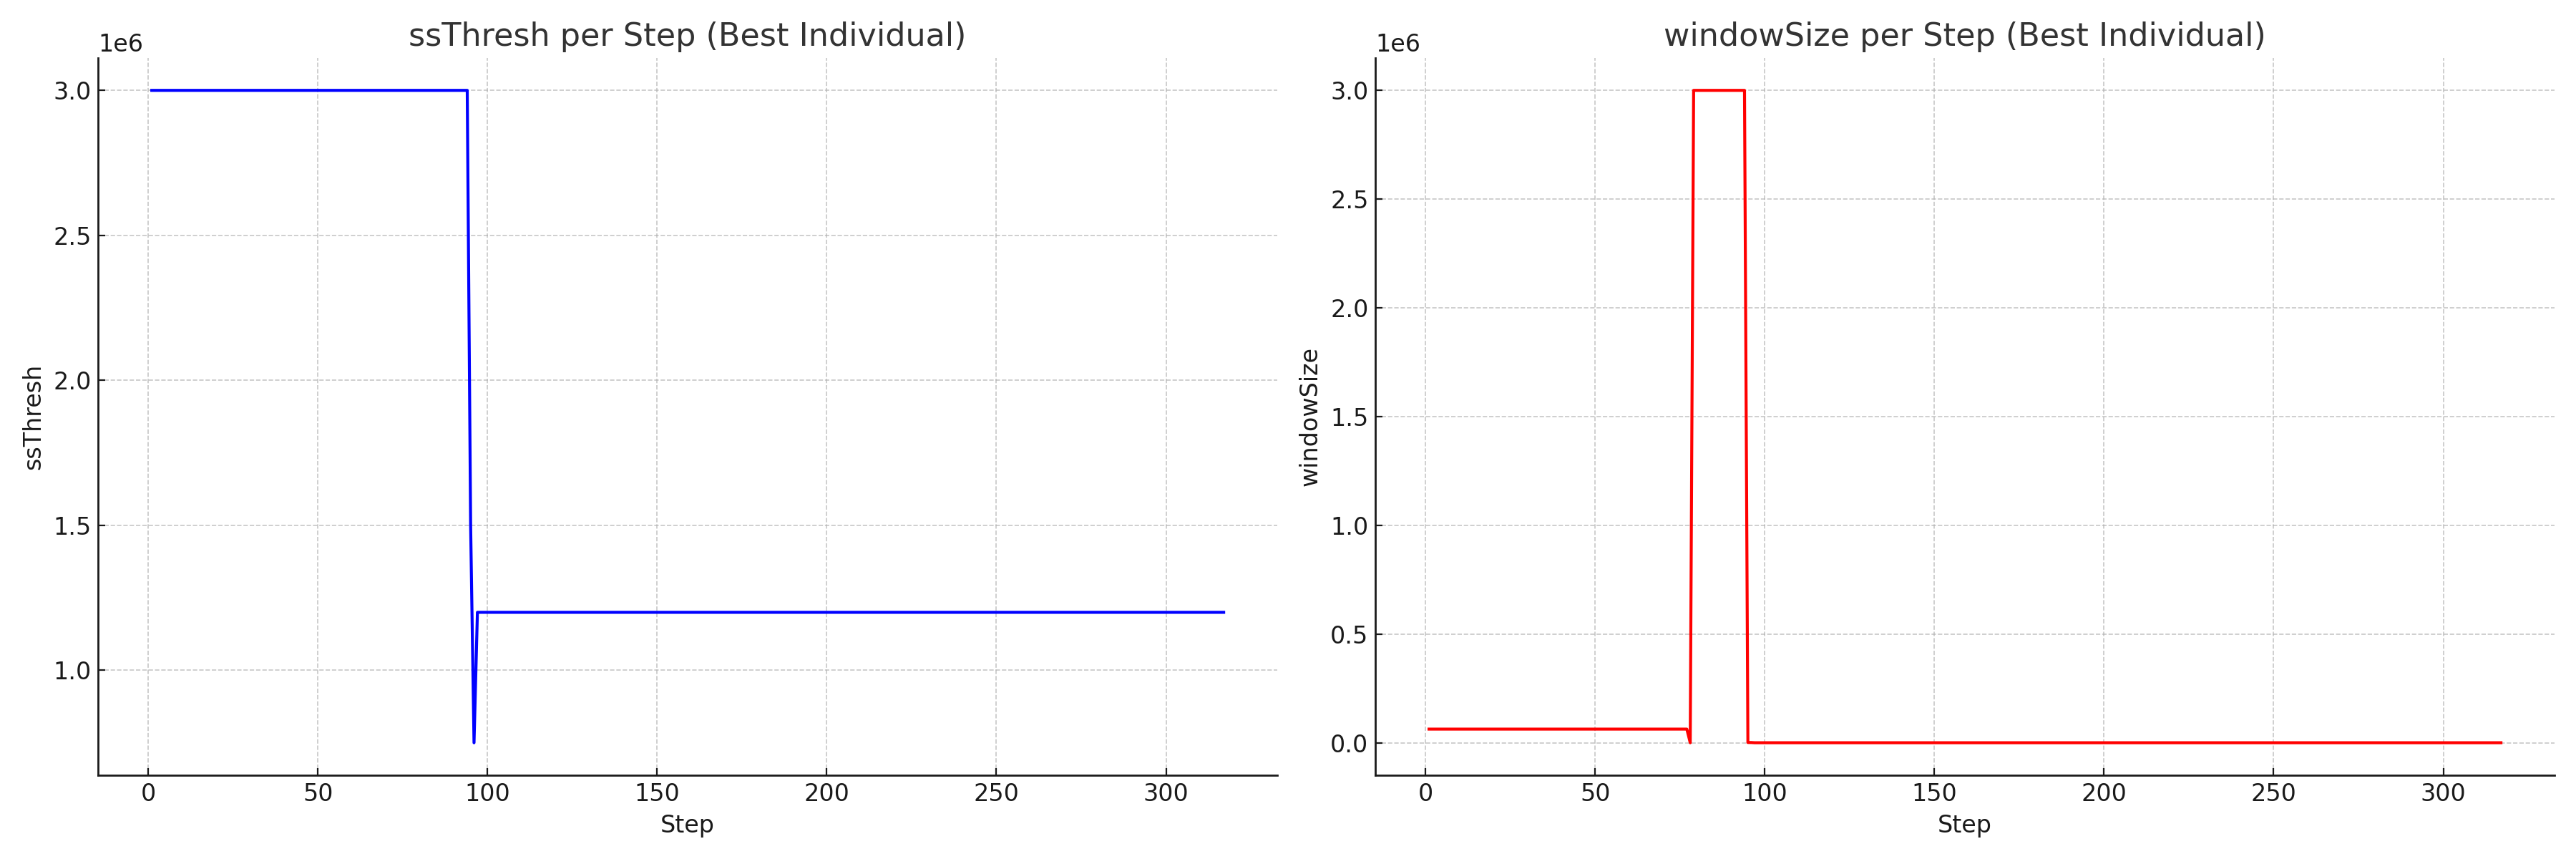
\includegraphics[width=1.0\linewidth]{fig/chap05/best_result.png}
  \caption{最もスループットが高かった個体のssthresh, cwndの推移}
  \label{figure:best_individual_result}
\end{figure}
また、ベンチマークとして用いたTCP NewRenoのssthresh, cwndの推移を\figref{figure:newreno_result}に示す。
\begin{figure}[htbp]
  \centering
  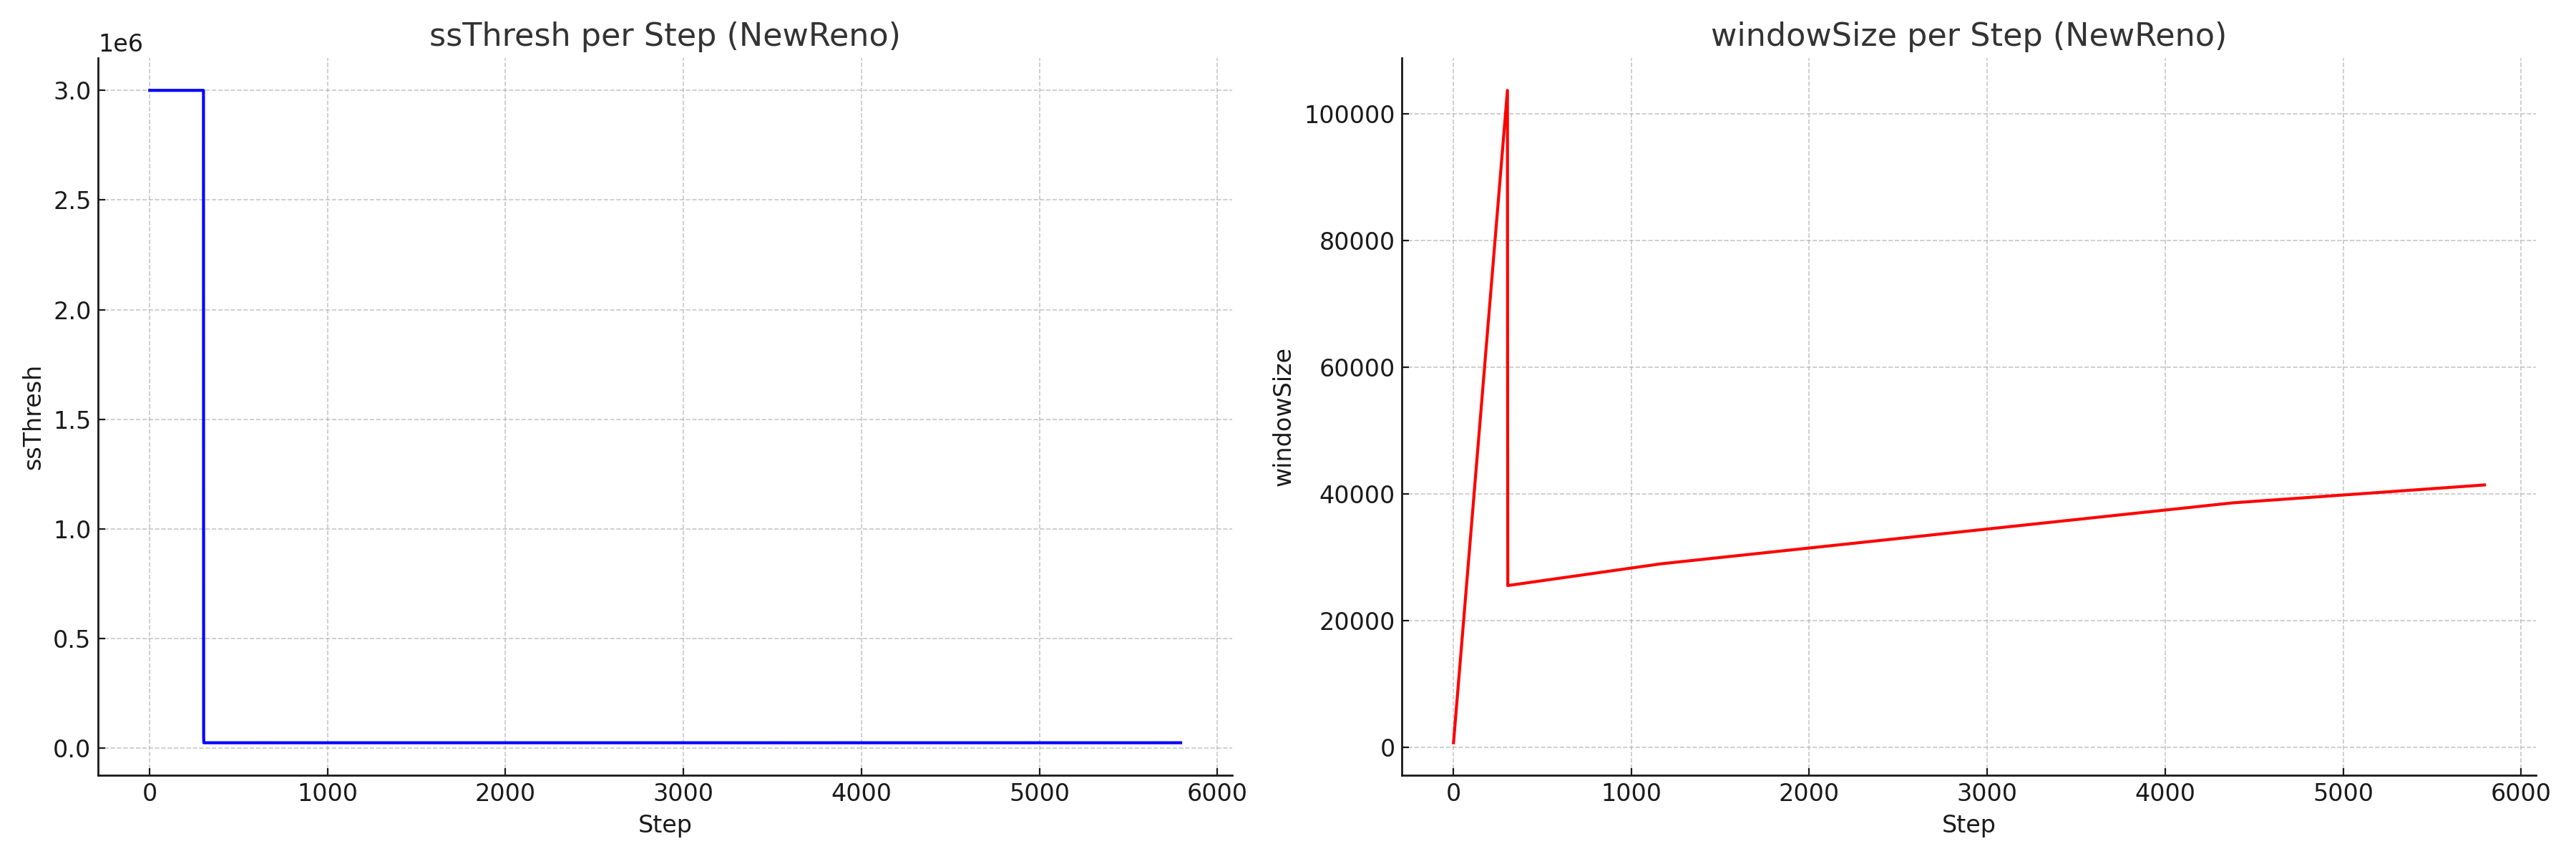
\includegraphics[width=1.0\linewidth]{fig/chap05/newreno_result.png}
  \caption{TCP NewRenoのssthresh, cwndの推移}
  \label{figure:newreno_result}
\end{figure}

なお、Listings \ref{lst:best_individual}のソースコードに関する詳細な議論は\chapref{chapter:discussion}であらためて行う。

\newpage

\chapter{考察}
\label{chapter:discussion}
この章では、\chapref{chapter:result}で示した結果について考察する。
特に、Listings \ref{lst:best_individual}に示した評価値の良い個体について、著名な輻輳制御アルゴリズムと比較しながら議論する。また、\chapref{chapter:hypothesis}で立てた仮説の検証という観点から、本研究の貢献について述べる。

\section{評価値の良い個体に関する考察}
議論の簡単のため、Listings \ref{lst:best_individual}に示した個体の疑似コードを\algorithmref{algorithm:highest-throughput-individual}に示す。
\begin{algorithm}
  \caption{Highest Throughput Individual Pseudocode}
  \label{algorithm:highest-throughput-individual}
  \begin{algorithmic}[1]

  \Procedure{get\_action}{$obs, reward, done, info$}
      \State Extract $ssThresh, cWnd, segmentSize, segmentsAcked, bytesInFlight$ from $obs$

      \If{$reward > 0$ \textbf{and} $segmentsAcked > 0$}
          \If{$cWnd < ssThresh$}
              \State $new\_cWnd \gets (cWnd^3 + segmentSize)^{\frac{1}{3}}$
          \Else
              \State $new\_cWnd \gets cWnd + (segmentSize \times segmentsAcked)$
          \EndIf
          \State $new\_ssThresh \gets \max(ssThresh, \lfloor bytesInFlight \times 0.8 \rfloor)$
      \Else
          \State $new\_cWnd \gets \lfloor \sqrt{bytesInFlight} \rfloor$
          \State $new\_ssThresh \gets \max(new\_cWnd, \lfloor ssThresh / 2 \rfloor)$
      \EndIf

      \State \textbf{return} $[new\_ssThresh, new\_cWnd]$
  \EndProcedure

  \end{algorithmic}
\end{algorithm}
\algorithmref{algorithm:highest-throughput-individual}を観察すると、現在広く普及している輻輳制御アルゴリズムの1つであるCUBIC\cite{cubic}やTCP NewReno\cite{floyd2004newreno,henderson2012newreno}の要素を部分的に取り入れつつも、ユニークなアルゴリズムを実現していると考えられる
\footnote{これはあくまでも、\algorithmref{algorithm:highest-throughput-individual}が著名な輻輳制御アルゴリズムの要素を部分的には取り入れつつも、それらのユニークな組み合わせや、そこにオリジナリティがあるという意味である。}。
具体的には、Listings \ref{lst:best_individual}のL.5では、CUBICのように、cwndの増加を立方関数で表現している
\footnote{厳密にはこの三乗根を取っているため、CUBICと同様の挙動を示すわけではない}。
また、L.7では、TCP NewRenoのようにcwndの増加を線形関数で表現している。

\section{仮説の検証}

\chapref{chapter:hypothesis}で立てた仮説は、以下の3つである。
\begin{enumerate}
  \item 大規模言語モデルを用いた輻輳制御アルゴリズムの探索手法は、既存の探索手法と比べて、探索空間が広がるのではないか
  \item 進化アルゴリズム、特に遺伝的アルゴリズムを用いることで、既存の探索手法よりも多様かつ優れた輻輳制御アルゴリズムを発見できるのではないか
  \item 1, 2で提案した探索手法であれば、任意のネットワーク環境下で最適な輻輳制御アルゴリズムを発見できるのではないか
\end{enumerate}
第一に探索空間の広がりについて考える。
\secref{subsection:evolutionary-algorithm}で述べたとおり、既存の探索手法では、探索空間が厳しく制限されてしまう。
これは、ソースコードを構文木によって表現し、交叉や変異を構文木に対する操作として定義しているためである。つまり、この操作を超えた探索を行うことはできず、ソースコード自体の構造を変化させるような探索は行えない。

一方本研究で提案した、大規模言語モデルを用いた探索手法では、ソースコードを文字列として表現し、交叉や変異を文字列に対する操作として定義している。
それゆえ、理論上は任意の文字列を生成できるため、探索空間の制約はなくなったと考えられる。
しかし、探索効率という観点では、まだ改善の余地があると考えられる。
\chapref{chapter:result}の\figref{figure:invalid_results}からも読み取れるように、実行不可能な個体が多く生成されていた。
また、\figref{figure:generation_throughput}や\figref{figure:generation_result_exclude_zero}からも読み取れるように、交叉や変異といった、遺伝的操作はうまく機能していない可能性がある。
交叉や変異の設計の改善や、別の進化アルゴリズムとの組み合わせなど、今後の展望があると考えられる。

第二に、探索された輻輳制御アルゴリズムの多様性について考える。
多様性の評価については難しく、本研究の中では定量的に評価できなかった。
例えばcwndやssthreshの分散、あるいは評価値の分散などを多様性の指標として用いることはできる。
しかし、これらの指標は、本実験の評価関数に依存していることや多くの場合、これらの値が大きいほど優れている傾向にあることから、多様性の指標としては適切ではないと考えられる。
例えば、\secref{section:congestion_control_algorithm_evaluation}であげた、公平性を用いた評価指標や、探索を行うネットワーク環境とは異なるネットワーク環境での評価指標を用いることで、多様性の評価を行うことは可能であると考えられる。

最後に、本研究の提案手法は任意のネットワーク環境下で最適な輻輳制御アルゴリズムの探索を行えるのか考える。
本実験を通じて一定の制約の下では、大規模言語モデルを用いた探索手法による輻輳制御アルゴリズムの探索が可能であることが示された
\footnote{もちろんその探索効率は、まだ改善の余地があると考えられる}。
ただし、大きく以下の3つの制約がある。
\begin{enumerate}
  \item ネットワーク環境をシミュレータ上で再現できること
  \item 探索においてLoss-based/Delay-basedの分類を超えないこと
  \item 評価関数が定義できること
\end{enumerate}
1, 2の制約は、評価のためにネットワークシミュレータを用いる必要があることに起因する。
Loss-basedとDelay-basedでは、輻輳の検出方法が全く異なるため、この分類を超えて探索することは難しいだろう
\footnote{例えば、初期個体にこれらを混在させることはできるかもしれないが、シミュレーションシナリオや評価関数の設計、交叉や変異の実装や、探索効率を考えると難しいだろう。
マルチエージェントシステムの観点から、例えばノード1をLoss-based、ノード2をDelay-basedとして、それぞれ探索を行うような試みは面白いかもしれないが、本稿ではこれ以上扱わない}。

またBBRのような、ネットワーク全体のボトルネックを推定するアルゴリズムについても、これらの問題から探索は難しいだろう。
評価関数の定義については、\secref{section:evaluation-method}で述べたとおり、本実験ではスループットを用いた。
しかし、実際の輻輳制御アルゴリズムの評価には、スループット以外にも様々な指標が用いられる。
例えば本実験では、ネットワーク全体の公平性を損ねてでも、パケットを送り続けるアルゴリズムが評価値の高い個体となる可能性がある。
このような問題に対処するためには、評価関数をより複雑にする必要がある。
輻輳制御アルゴリズムの性能評価については、\secref{section:congestion_control_algorithm_evaluation}でも概説したが、支配的な輻輳制御アルゴリズムが存在しないことと同様に、決定的な評価指標はいまだに存在しない。
評価指標の設計は、今後改良の余地があると考えられる。

\section{本研究の貢献}
\label{section:contribution}

章の最後に、本研究の貢献について述べる。
従来、輻輳制御アルゴリズムの探索手法としては、分散最適化のアプローチによるものや、メタヒューリスティクスによるものが多かった。
これらの探索手法から派生して、Endoら\cite{endo-2022-toward}は、進化アルゴリズムを用いた輻輳制御アルゴリズムの探索手法を提案した。
しかしEndoらの手法では、ソースコードを構文木によって表現し、交叉や変異を構文木に対する操作として定義していたため、探索空間に大きな制約があった。

本研究では、この探索空間の制約を解消するために、大規模言語モデルを用いた探索手法を提案した。
大規模言語モデルを用いて進化演算を行うため、原理的には任意の輻輳制御アルゴリズムを生成できる。
提案手法を用いることで、既存の探索手法では発見が不可能であった個体を発見できる可能性がある。

\newpage

\chapter{まとめ}

本研究のまとめと今後の展望について述べる。
\secref{section:contribution}で述べたとおり、既存の輻輳制御アルゴリズムの探索手法では、探索可能なアルゴリズムが限られていた。
これは、輻輳制御アルゴリズムを表すソースコードの表現方法に起因するものであった。
本研究では、ソースコードを文字列として表し、大規模言語モデルを用いて進化演算を行うことで、この制約を解消した。
実際にネットワークシミュレータを用いた探索実験を行い、広く使われている輻輳制御アルゴリズムよりも高い性能を示す個体を発見できた。
今回発見された個体は、既存の探索手法では発見できなかったものであり、これが本研究の貢献である。

しかし、いくつかの課題も残されている。
\chapref{chapter:discussion}で述べたとおり、遺伝的アルゴリズムの交叉や変異が、十分に機能していない可能性がある。
これは世代を追っても評価値の平均が上昇しなかったことからも読み取れることであり、探索効率の観点で、改善の余地があると考えられる。
また、シミュレーションを行ったネットワーク環境や、遺伝的アルゴリズムに与えるパラメータ
\footnote{例えば交叉率や変異率、個体数など}
、大規模言語モデルへのパラメータ
\footnote{例えばトークン数やモデルのサイズ、温度など}
プロンプトの設計など、探索の際のチューニングの余地がある。
評価指標についても、本実験ではスループットを用いたが、他にも様々な指標が考えられる。
輻輳制御アルゴリズムの性能評価自体が依然大きな課題であるゆえ、評価指標の設計についても改善の余地があると考えられる。

今後は、これらの課題に対処することや、他の進化アルゴリズムとの組み合わせなどによって、探索効率の向上につながるような改良を行いたい。
また、発見した個体を実際のネットワーク環境で評価することで、本研究の有用性を検証したい。

\chapter*{謝辞}
\addcontentsline{toc}{chapter}{\numberline{}謝辞}

本研究を行うにあたって、研究テーマの決定、研究内容の議論、外部発表の機会の提供など、様々な形でご指導を頂いた岡瑞起准教授、阿部洋丈准教授の両先生に深く感謝を申し上げます。
また、同研究プロジェクトの中で議論した、岡研究室の矢内千陽さん、OSSS研究室の佐藤創太さんの両氏にも感謝を申し上げます。
ネットワークシミュレータの取り扱いや実験環境に関して、OSSS研OBの森越さんには多大なるご協力を頂きました。
実験用のマシンのセットアップ等に関して、OSSS研の山本さん、広瀬さんには大変お世話になりました。
この場を借りて、深く御礼申し上げます。

そして、日々の研究活動やミーティングにおいて、様々な形でご協力を頂いた岡研究室の皆様、OSSS研究室の皆様にもあらためて感謝申し上げます。

\newpage

\addcontentsline{toc}{chapter}{\numberline{}参考文献}
\renewcommand{\bibname}{参考文献}

\bibliographystyle{junsrt}
\bibliography{ref.bib}

\appendix
\chapter{実験結果の詳細}
\label{appendix:experiment-result}
実験の結果、もっともスループットが高かった個体のソースコードをListings \ref{lst:best_individual}に示す。
\begin{lstlisting}[caption=最もスループットが高かった個体のソースコード,label=lst:best_individual]
  from tcp_base import TcpEventBased

  class TcpEventBase(TcpEventBased):
      def __init__(self):
          super(TcpEventBased, self).__init__()

      def get_action(self, obs, reward, done, info):
          # unique socket ID
          socketUuid = obs[0]
          # TCP env type: event-based = 0 / time-based = 1
          envType = obs[1]
          # sim time in us
          simTime_us = obs[2]
          # unique node ID
          nodeId = obs[3]
          # current ssThreshold
          ssThresh = obs[4]
          # current contention window size
          cWnd = obs[5]
          # segment size
          segmentSize = obs[6]
          # number of acked segments
          segmentsAcked = obs[7]
          # estimated bytes in flight
          bytesInFlight = obs[8]

          # Mutate the congestion window and ssThreshold calculation
          if reward > 0 and segmentsAcked > 0:
              # Aim for cubic growth until ssThresh and linear afterwards
              new_cWnd = (
                  (cWnd**3 + segmentSize) ** (1 / 3)
                  if cWnd < ssThresh
                  else cWnd + (segmentSize * segmentsAcked)
              )
              new_ssThresh = max(ssThresh, int(bytesInFlight * 0.8))
          else:
              # Quick recovery using a square root
              new_cWnd = int(bytesInFlight**0.5)
              new_ssThresh = max(new_cWnd, ssThresh // 2)

          # return actions
          actions = [int(new_ssThresh), int(new_cWnd)]

          return actions
  \end{lstlisting}

\end{document}
